\chapter{Methodology}
\label{Methodology}


\section{Software and Hardware}
\todo{write this}

For certain specialized tasks, such as PET SUV calculation and RTstruct conversion, parts of source code from a public repository \footnote{\url{https://github.com/voreille/hecktor}} were used to ensure the correctness of the implementation. This code repository contains utility code created as part of the HECKTOR PET/CT segmentation challenge \cite{andrearczyk2020overview} by its authors.

% FDG SUV calculation
For the sake of correctness of the implementation of this formula, utility code from the HECKTOR repository was used to perform this conversion \footnote{BQML to SUV conversion code: \url{https://bit.ly/33IG4Jg}}.




%%%%%%%%%%%%%%%%%%%%%%%%%%%%%%%%%%%%%%%%%%%%%%%%%%%%%%%%%%%%%%%%%%%%%%%%%%%%%%%%%%%%%%%%%%%%%%%%%%%%%%%%%%%%%%%%%%%%%%%%%%%%%%%%%%%%%%%%%%%%%%%
\section{Data}
% Image modalities involved and their properties
% The Maastro Lung HX4 dataset
% Data processing
The medical imaging dataset used in this project, hereafter referred to as \textit{Maastro Lung HX4 dataset}, is a combination of two different datasets originally acquired for two clinical trials at Maastro, and was also previously used by Even et al. \cite{even2017predicting} in their hypoxia prediction study. It includes 3D scans of 34 Non-Small Cell Lung Cancer (NSCLC) patients in total, of which 15 belong to the \textit{PET-Boost} trial (registration number NCT01024829) \cite{van2012pet} and 19 to the \textit{Nitroglycerin} trial (registration number NCT01210378) \cite{even2017predicting}. The request for the usage of this data in this project was approved by the institutional review board (IRB).


% -------------------------
\subsection{Original Scans}
\label{Original_Scans}
In the original dataset, each individual scan was stored as a separate DICOM series \footnote{DICOM is an international standard for storing and managing medical images: \url{https://www.dicomstandard.org/}} which contained the image intensity data, the spatial information of the image and the image acquisition details. The first set of images for each patient included the Planning FDG-PET/CT images, where the CT component was the radiotherapy treatment planning CT (pCT). Both images were acquired using a single hybrid scanner and were, hence, registered with each other by default. The 3D field-of-view (FOV) of both images included the patient's chest, although the FOV of pCT was different than that of FDG-PET. Spatial resolution of all FDG-PET images was 4$\times$4$\times$3 mm$^3$ and that of the pCT was 0.97$\times$0.97$\times$3 mm$^3$, specified in the \textit{x}$\times$\textit{y}$\times$\textit{z} format. Additionally, annotations of certain structures relevant to the treatment planning process, for example, the primary tumor, nearby organs-at-risk, and the patient's body, were provided for each patient in the DICOM \textit{RTstruct} format \footnote{Radiotherapy structure set (RTstruct) is the DICOM-specified format for storing radiotherapy-related annotations: \url{https://dicom.innolitics.com/ciods/rt-structure-set}}. These structures were delineated by a radiation oncologist on the Planning CT (pCT). Figure \ref{fig:original_fdgpet_pct} shows a visualization of FDG-PET and pCT images of a sample patient.

\begin{figure}[h!]
    \centering
    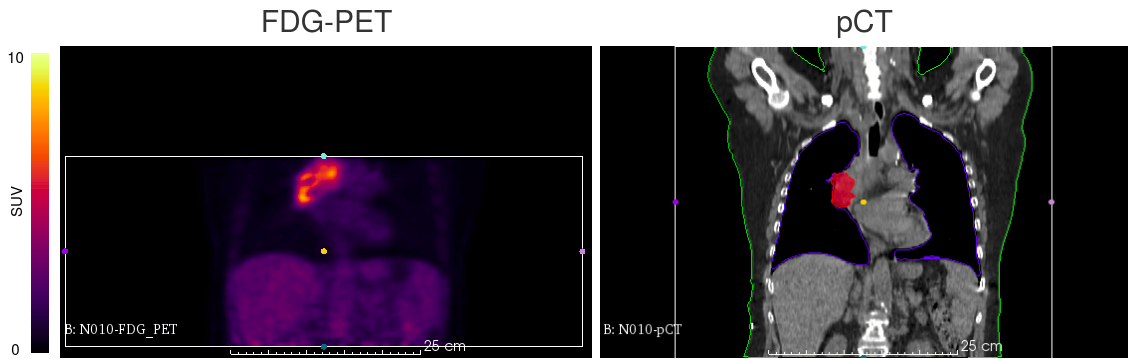
\includegraphics[width=\linewidth]{figures/Data/original/N010-FDG_PET_pCT.png}
    \caption{Single coronal (\textit{x}-\textit{z} plane) slice of FDG-PET and pCT images. White bounding boxes show their respective FOVs. Radiotherapy structure annotations were provided for pCT of which three are shown here -- the patient's body (green), the lungs (dark blue) and the primary tumor (red). FDG-PET shows high activity near the tumor region.}
    \label{fig:original_fdgpet_pct}
\end{figure}

The second set of images included the HX4-PET and the accompanying low-dose CT (ldCT). For each patient, these were acquired on a different day than their corresponding FDG-PET/pCT scans. Both images were simultaneously acquired (thus, aligned with each other by default), and they cover approximately the same FOV of the patient's chest. However, the FOV covered by HX4-PET/ldCT couple was more focused on the tumor and was smaller in the axial direction compared to the FDG-PET/pCT couple. The HX4-PET images had a resolution of 4$\times$4$\times$4 mm$^3$ and the resolution of ldCT was 1.17$\times$1.17$\times$4 mm$^3$. Figure \ref{fig:original_hx4pet_ldct} shows a visualization of sample HX4-PET and ldCT images.

\begin{figure}[h!]
    \centering
    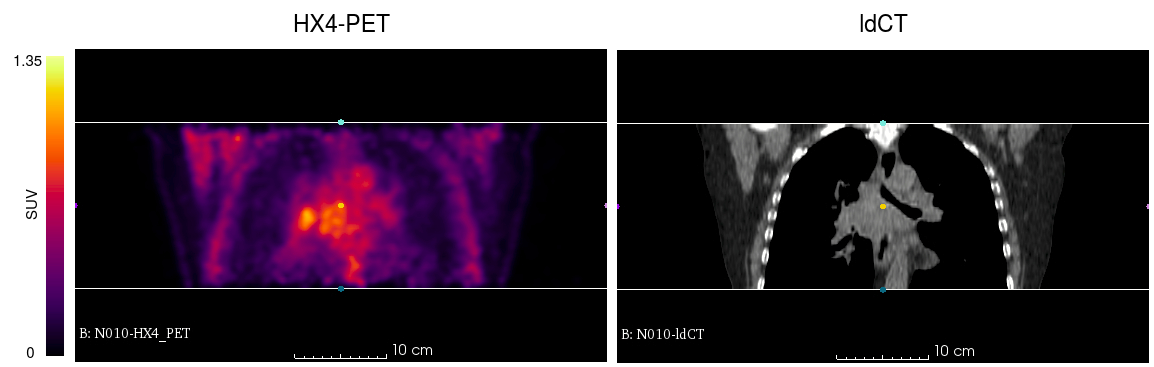
\includegraphics[width=\linewidth]{figures/Data/original/N010-HX4_PET_ldCT.png}
    \caption{Single coronal slice of HX4-PET and ldCT images. Both had similar FOVs. No annotations were provided for the ldCT.}
    \label{fig:original_hx4pet_ldct}
\end{figure}

Both the CT images -- pCT and ldCT -- had their voxel intensity values expressed in terms of the Hounsfield Unit (HU), which is related to the radiodensity of materials. In case of FDG-PET, the units represent levels of radioactivity emitted from the FDG tracer in different parts of the body as measured by the scanner, and were represented in terms of Becquerel per milliliter (Bq/mL, abbreviated as BQML). In HX4-PET, however, intensities were expressed in terms of a different unit called \textit{counts} (abbreviated as CNTS). This unit is specific to the manufacturer, and possibly also to the model, of the PET/CT scanner (Philips Gemini TF64) that was used for HX4-PET acquisition. Before using them for any purpose, FDG-PET and HX4-PET needed their intensity values to be converted to Standardized Uptake Values (SUV) which is the standard unit for PET intensity representation. SUV calculation is discussed in further detail in \ref{data_proc_phase_1}.


% -----------------------------
\subsection{Image Registration}
Note that although each of the two PET/CT couples -- FDG-PET/pCT and HX4-PET/ldCT -- had the PET and CT components aligned with each other by default, both PET/CT couples did not align organ-to-organ with \textit{each other} because they had different \textit{physical} reference frames due to both being acquired in different scanning sessions. Having a version of HX4-PET that is registered to the FDG-PET/pCT was essential to serve as a ground-truth image for evaluating the GANs as well as for paired training of Pix2Pix. Even et al. \cite{even2017predicting} describe a registration procedure for achieving this alignment. They use a two-step approach where the ldCT is first subjected to rigid alignment followed by non-rigid elastic registration over the pCT. The resulting transformation parameters are then applied to the HX4-PET image. Figure \ref{fig:reg_images} shows an example of HX4-PET image before and after registration. 

\begin{figure}[h!]
    \centering
    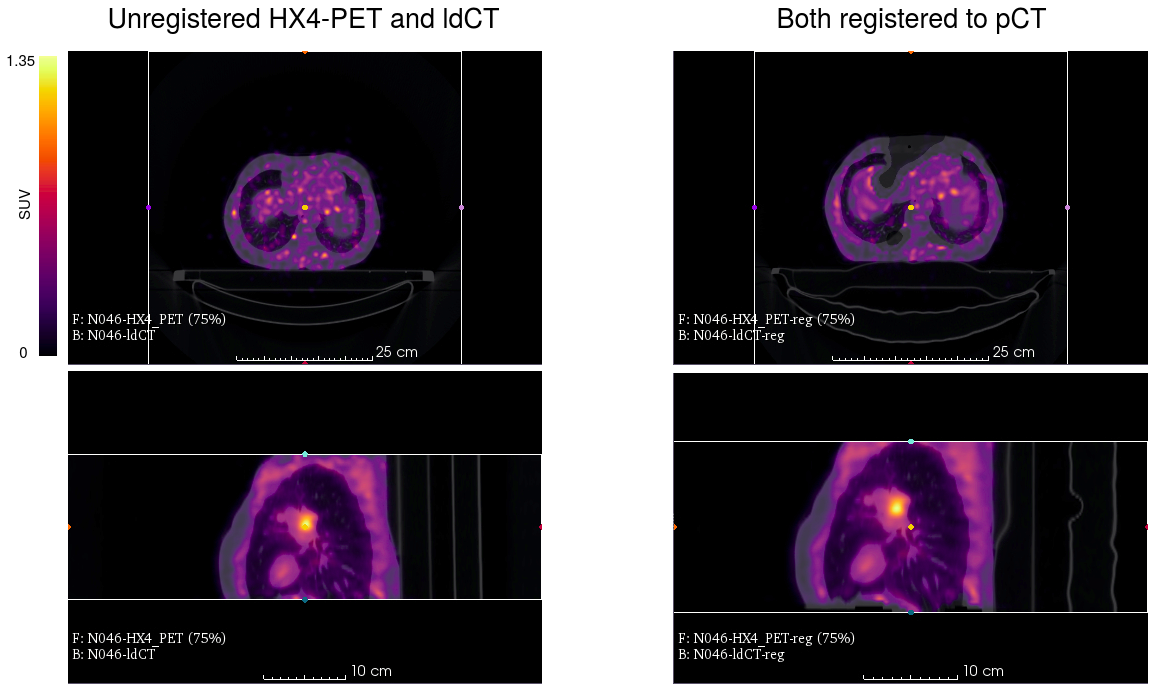
\includegraphics[width=\linewidth]{figures/Data/reg/N046-HX4_PET_ldCT-unreg_reg.png}
    \caption{Overlaid HX4-PET and ldCT images of a patient before and after registration to pCT, showing axial (top) and sagittal (bottom) slices. pCT is not shown. The scanner table is visible in the ldCT background, and shows the effects of the elastic transformation. Some registration errors are observed here. For example, in the axial slice, the HX4-PET region close to the patient's top surface is overly warped towards the inside resulting in an empty region of zero intensity. Also, in the sagittal slice in (b), some voxels at the bottom are missing the hypoxia signal due to warping.}
    \label{fig:reg_images}
\end{figure}{}

The Maastro Lung HX4 dataset already included the registered HX4-PET and ldCT images, and therefore this registration step wasn't needed to be performed. These images were supplied in the \textit{.mhd/.raw} format. The intensity values of the stored registered HX4-PET were expressed in SUVs, supposedly calculated before the registration process. 

To distinguish the registered HX4-PET from the unregistered one, the two are denoted as \textit{HX4-PET-reg} and \textit{HX4-PET-unreg}, respectively. The term \textit{HX4-PET} is used hereafter to denote the image modality in a general sense and not referring to the registered or unregistered versions of the images from the dataset. It is obvious that FDG-PET and pCT were needed since both would be the inputs to the GANs, and HX4-PET-reg to be the ground-truth given these inputs. And since HX4-PET-reg contained registration imperfections as seen in Figure \ref{fig:reg_images}, the HX4-PET-unreg instead would be used in the unpaired CycleGAN training to sidestep this issue. The \textit{unregistered} ldCT, \textit{ldCT-unreg}, would play a crucial role in the modified CycleGAN system as discussed further in \ref{data_requirements}, and hence was not discarded. However, the \textit{registered} ldCT wouldn't be required anymore beyond this point since its sole purpose was to aid in the registration of HX4-PET, and was thus discarded.


% --------------------------------
\subsection{Data Processing Steps}
\label{Data_Processing}
The Maastro Lung HX4 dataset needed to be prepared and converted into a form that could be used for GAN training. The different processing steps performed on the data are discussed here. The overall data processing can be broken down into two phases, which are elaborated in the following paragraphs. 

\subsubsection{Loading Images and Converting to Appropriate Representation}
The first step was to load the images from different formats into computer memory and convert to a standard programmatic representation. All the original images, except for HX4-PET-reg, were supplied as DICOM series. 

\vspace{4mm}
\noindent
\textit{SUV Calculation:} First, The FDG-PET and HX4-PET-unreg intensity values needed to be converted into the SUV scale. When the intensity units are expressed as BQML, as with all FDG-PET images here, the patient's body weight as well as imaging parameters including the decay time and the total administered dose of the radiotracer are required to calculate the SUV. Equation \ref{BQML_to_SUV} shows the conversion formula. 
\begin{equation}
    SUV = \frac{BQML * 1000 * Weight}{Dose * 2^{-t/\tau}} 
    \label{BQML_to_SUV}
\end{equation}
where $2^{-t/\tau}$ is the decay correction factor at time of acquisition \textit{t}, given the half-life $\tau$ of the radiotracer. The values for the patient's weight, administered dose and decay parameters are stored in the DICOM image series as metadata, which was accessed using the PyDicom library. 

HX4-PET-unreg images, however, were represented in terms of the non-standard CNTS units here, for reasons discussed earlier in \ref{Original_Scans}. CNTS to SUV conversion was performed using the formula implemented in this \footnote{CNTS to SUV conversion code: \url{https://bit.ly/3wbtGgW}} public GitHub repository.

\vspace{4mm}
\noindent
\textit{Conversion of RTstruct Contours to Binary Masks:} RTstruct is the format defined in the DICOM standard for storing radiotherapy-related annotations (known as "radiotherapy structure sets") in the form of contour points. The RTstruct file is stored separately from the scans. Since the process of radiotherapy treatment planning involves creating these contours over the Planning CT (pCT), the physical coordinate system of the pCT scan is the reference frame for the contour points. Of all the different objects annotated in the pCT scan, only the contours for the primary tumor and the patient's body were selected and converted to binary masks. Each of these masks have the same 3D size and resolution as the pCT image. The tumor mask would be needed during evaluation of the hypoxia maps predicted by the models, whereas the body mask would be required during their training to mask away and remove out-of-body objects in scans, for example, the scanner table. The algorithm implemented in this \footnote{RTstruct to binary mask conversion code: \url{https://bit.ly/2RnNI9t}} GitHub repository was used to perform the RTstruct-to-binary-mask conversion.

\begin{figure}[h!]
    \centering
    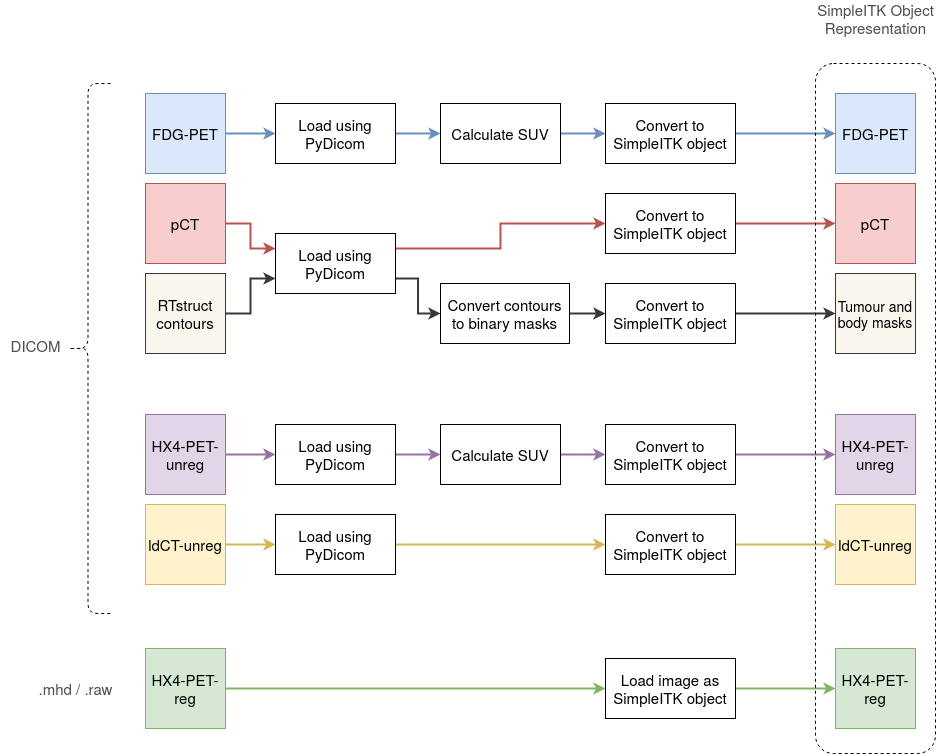
\includegraphics[width=0.9\linewidth]{figures/Data/data_processing_overview-step_1.png}
    \caption{Overview of the first phase of data processing. Images were loaded from storage into computer memory in a standard programmatic representation.}
    \label{fig:data_proc_overview_1}
\end{figure}

Following this, the FDG-PET, HX4-PET-unreg, pCT and the tumor and body masks were converted to SimpleITK objects in Python. The ldCT-unreg was also loaded using PyDicom and converted to this representation. HX4-PET-reg, stored in \textit{.mhd/.raw} format containing pre-computed SUV values, was directly loaded into a SimpleITK object. Figure \ref{fig:data_proc_overview_1} shows a visual overview of these steps.


\subsubsection{Cropping and Resampling}

\begin{figure}[h!]
    \centering
    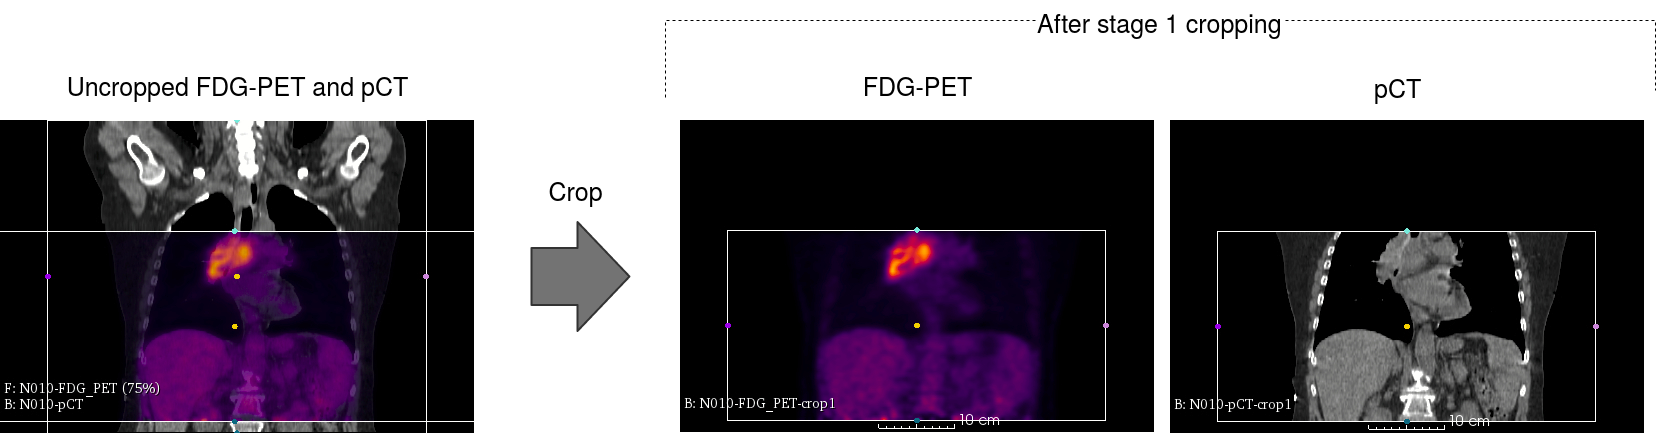
\includegraphics[width=\linewidth]{figures/Data/fdgpet_pct_crop1/N010-FDG_PET_pCT-uncropped_crop1.png}
    \caption{Stage 1 cropping of FDG-PET, pCT and the tumor and body masks (not shown here) to a common FOV. Uncropped FDG-PET and pCT are overlaid to show the overlap of their FOVs.}
    \label{fig:fdg_pet_pct_crop1}
\end{figure}

\begin{figure}[h!]
    \centering
    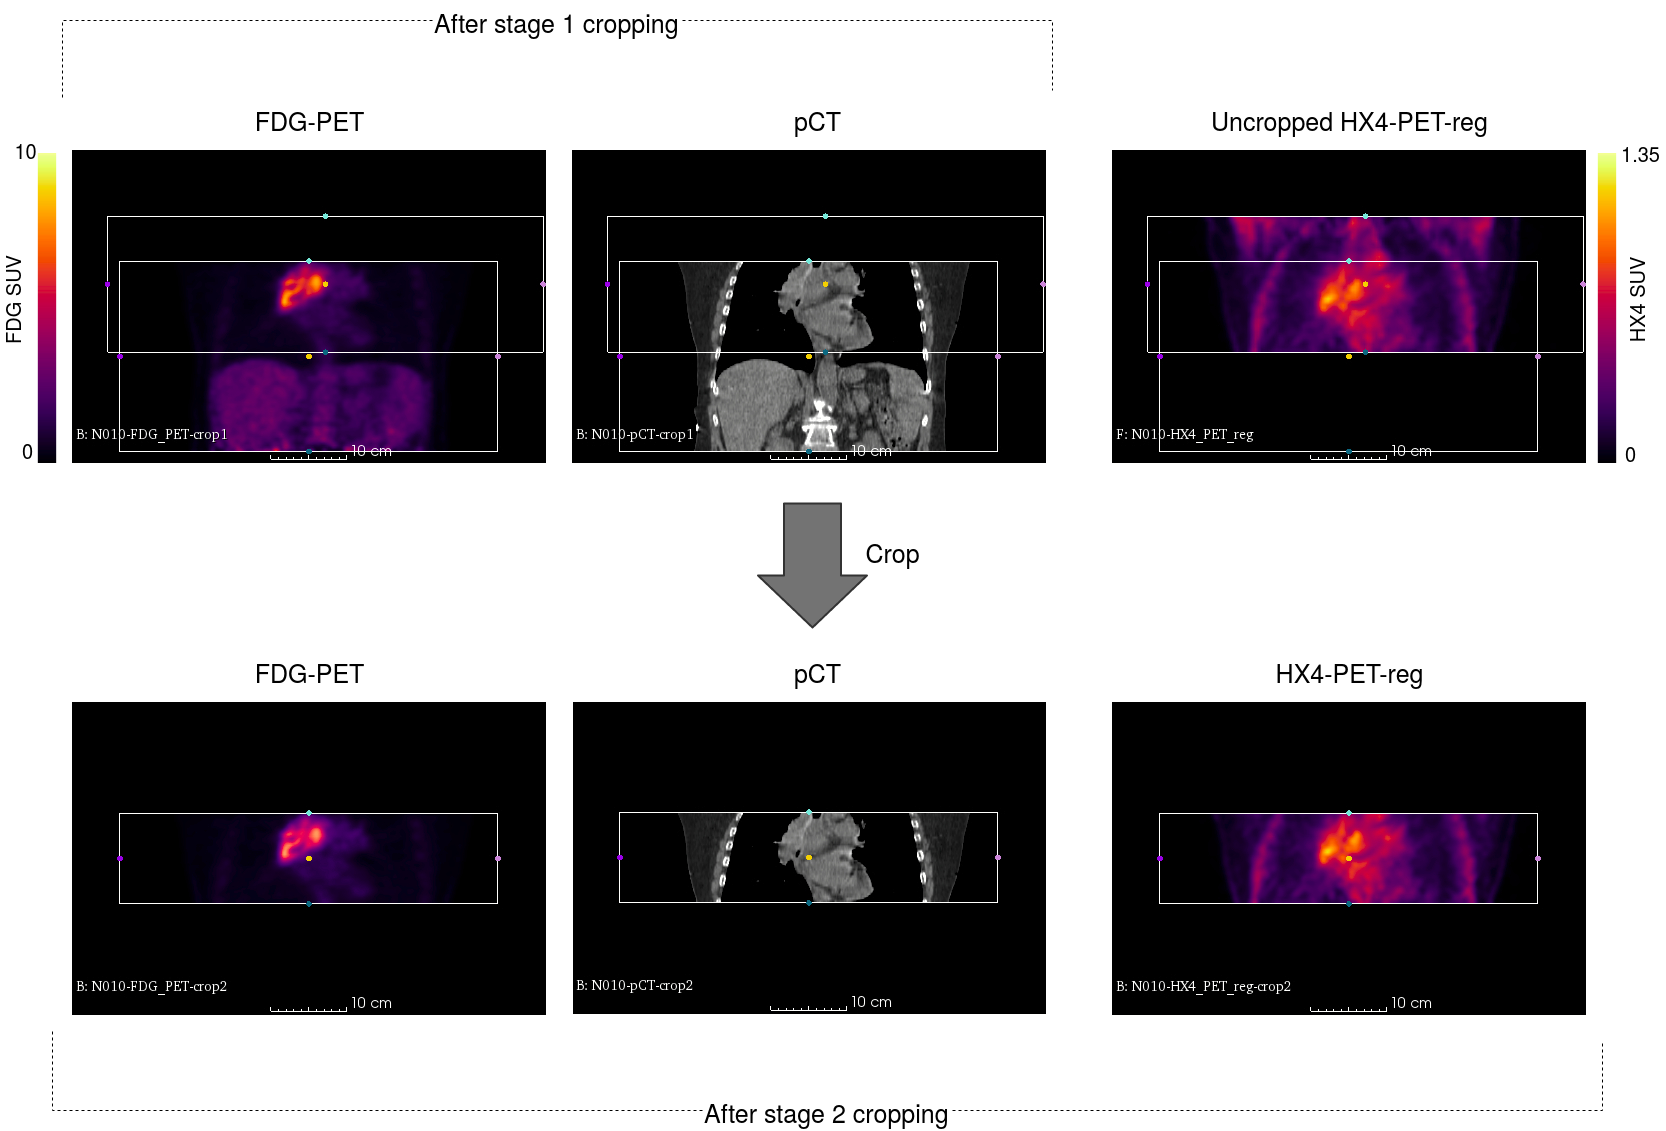
\includegraphics[width=\linewidth]{figures/Data/fdgpet_pct_fx4petreg_crop2/N010-fdgpet_pct_hx4petreg-uncropped_crop2.png}
    \caption{Stage 2 cropping of the input images (FDG-PET and pCT), the masks (tumor and body, not shown here) and the ground truth (HX4-PET-reg) to a common FOV. All FOVs are displayed to show their overlap.}
    \label{fig:fdgpet_pct_hx4petreg_crop2}
\end{figure}

The second data processing phase involved cropping and resampling the loaded images. A standard resampling resolution of 1$\times$1$\times$3 mm$^3$ was chosen. Cropping was performed in a progressive manner as described in the following steps: 

\begin{enumerate}
    \item \textit{Cropping and resampling FDG-PET, pCT and masks:} As shown earlier in \ref{Original_Scans}, the FOVs of FDG-PET and pCT are different. Both images needed to be cropped such that both would contain the same FOV of the patient. This can be solved by finding the 3D volumetric intersection of both their FOVs and cropping to this new volume size. The resampling step was performed immediately following this. The tumor and body masks share the same FOV with pCT, and hence, were cropped the same way as pCT was. This is the Stage 1 cropping of FDG-PET, pCT and the masks. Figure \ref{fig:fdg_pet_pct_crop1} illustrates this step.

    \item \textit{Cropping and resampling HX4-PET and ldCT:} The same process of cropping to common FOV followed by resampling was performed on HX4-PET-unreg and ldCT-unreg images. This is the Stage 1 cropping of HX4-PET-unreg and ldCT-unreg.

    \item \textit{Resampling HX4-PET-reg:} The HX4-PET-reg image was then just resampled to the standard resolution.

    \item \textit{Cropping the input images, the masks and the ground-truth image to common FOV:} Furthermore, the two input images (FDG-PET and pCT), the two masks and the ground-truth image (HX4-PET-reg) were cropped to the common FOV among them. The reason being that although HX4-PET-reg is organ-to-organ aligned with the input images and all of them have a common physical reference frame (due to registration), its FOV is different. This is the Stage 2 cropping. Figure \ref{fig:fdgpet_pct_hx4petreg_crop2} shows a visualization of this step.
\end{enumerate}

\begin{figure}[h!]
    \centering
    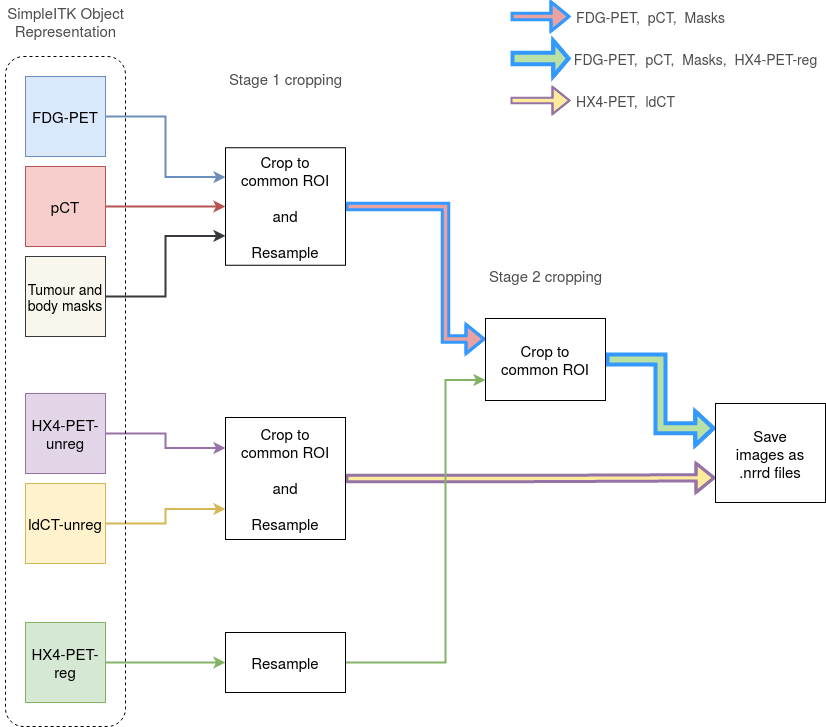
\includegraphics[width=0.8\linewidth]{figures/Data/data_processing_overview-step_2.png}
    \caption{Overview of the second phase of data processing.}
    \label{fig:data_proc_overview_2}
\end{figure}

Finally, all the processed images were saved as \textit{.nrrd} files. The NRRD format allows storage of N-dimensional raster images along with their spatial information, including voxel spacing (resolution) and physical coordinates of the origin, as a single file. Figure \ref{fig:data_proc_overview_2} shows an overview of the entire second phase of data processing discussed thus far. The dataset was then split into a training set and a validation set. The training set was comprised of data from the PET-Boost clinical trial (15 patients), and the validation set consisted of the data from the Nitroglycerin trial (19 patients). 



%%%%%%%%%%%%%%%%%%%%%%%%%%%%%%%%%%%%%%%%%%%%%%%%%%%%%%%%%%%%%%%%%%%%%%%%%%%%%%%%%%%%%%%%%%%%%%%%%%%%%%%%%%%%%%%%%%%%%%%%%%%%%%%%%%%%%%%%%%%%%%%
\section{GAN Systems}
\label{GAN_Systems}
This section describes the image translation GAN systems used in our study. Unless explicitly mentioned otherwise, domain \textit{A} is used throughout this section to represent the domain of valid multimodal FDG-PET/pCT images, and \textit{B} to represent the domain of HX4-PET images. Synthetic HX4-PET images are denoted as \textit{HX4-PET-syn}.


% ------------------
\subsection{Pix2Pix}
\label{pix2pix}
The Pix2Pix framework provides a simple and straightforward image translation method, provided the images in domain \textit{A} and domain \textit{B} in the training dataset are paired and have pixel-wise correspondence. The Pix2Pix generator is a deep neural network that takes as input an image and outputs an image of the same size, and the discriminator is a classifier network that takes image input and outputs a scalar value or a downsampled map of scalar values (see further in \ref{network_architectures}). For some \textit{A}-to-\textit{B} cross-domain translation task, it is first assumed that an \textit{A}-to-\textit{B} mapping exists. The generator models this relationship between the domains and the discriminator models the conditional probability that an image belongs to domain \textit{B}, given its counterpart from domain \textit{A}. During training, the generated domain \textit{B} images are evaluated by the conditional discriminator, and its adversarial feedback is used to improve the generator's performance. Additionally, Pix2Pix uses a pixel-wise loss to directly enforce similarity between the synthetic and the ground-truth domain \textit{B} images. For a generator $G$ and a discriminator $D$, Equation \ref{eq:pix2pix_loss_components} shows the components of each of their loss functions. 

\begin{equation}
    \begin{aligned}
    L(G) &= L_{adv}(G) + \lambda L_{elem}(G) \\
    L(D) &= L_{adv}(D)
    \end{aligned}
    \label{eq:pix2pix_loss_components}
\end{equation}
$G$ has two loss components -- an adversarial loss $L_{adv}(G)$ and an element-wise loss $L_{elem}(G)$. Loss for $D$ is a single adversarial loss $L_{adv}(D)$ which is a counterpart of $L_{adv}(G)$. In $G$, $L_{adv}(G)$ can be viewed as a ``structured" loss that is learned from the data itself as a result of the adversarial setting and can produce images with sharp and fine structures, whereas $L_{elem}(G)$ emphasizes on preserving larger and lower-frequency components of the images. The hyperparameter $\lambda$ can be used to adjust the balance of importance between the two terms depending on the specific application.

We use the least-squares version of the adversarial loss, instead of the original cross-entropy loss, as it is known to improve training stability \cite{mao2017least}. Similar to the original Pix2Pix framework \cite{isola2017image}, we implement $L_{elem}(G)$ as pixel-wise (voxel-wise in 3D) L1 loss. Equation \ref{eq:pix2pix_loss_expansion} shows the expansion of each of these loss terms.

\begin{equation}
    \begin{aligned}
    L_{adv}(G) &= E_{x \sim p_{data}(x)} [(1 - D(x, G(x)))^2]  \\
    L_{adv}(D) &= E_{x \sim p_{data}(x)} [D(x, G(x))^2] + E_{x,y \sim p_{data}(x,y)} [(1 - D(x,y))^2] \\
    L_{elem}(G) &= E_{x,y \sim p_{data}(x,y)} [|| y - G(x) ||_1]  \\
    \end{aligned}
    \label{eq:pix2pix_loss_expansion}
\end{equation}

where $x$ and $y$ are random variables representing samples from domain \textit{A} and \textit{B}, respectively, and the joint data distribution is denoted by $x,y \sim p_{data}(x,y)$. The adversarial objectives of $G$ and $D$ -- $L_{adv}(G)$ and $L_{adv}(D)$ -- are conflicting. For a given $D$, $G$ learns to synthesize images that $D$ would evaluate as real data samples (with a value of 1). Whereas, for a given $G$, $D$ learns to correctly distinguish between the synthetic samples (with a value of 0) and the real samples (with a value of 1). During training, $G$ and $D$ are updated in an alternating fashion.

\begin{figure}[h!]
    \centering
    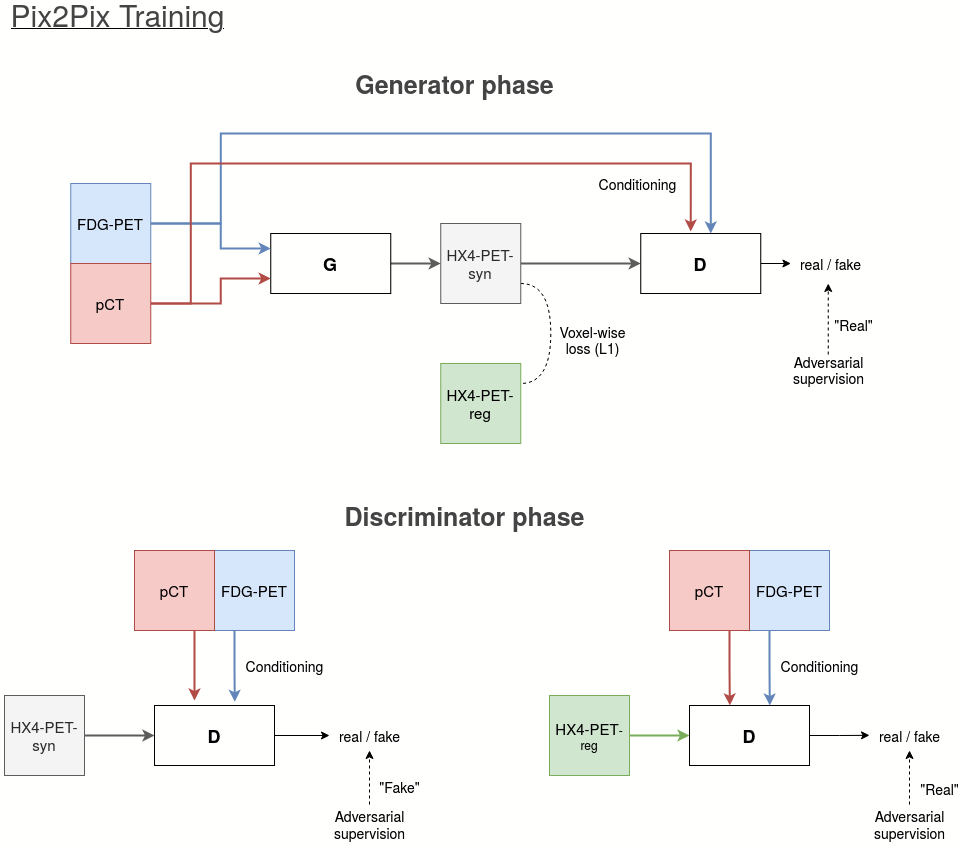
\includegraphics[width=\linewidth]{figures/GANs/Pix2Pix.png}
    \caption{Pix2Pix training phases. \textit{G} and \textit{D} are updated in an alternating manner. In practice, FDG-PET and pCT images were stacked channel-wise and given as input to \textit{G}. And in \textit{D}, the conditioning was implemented by channel-wise stacking the HX4-PET-reg or HX4-PET-syn with FDG-PET and pCT.}
    \label{fig:pix2pix}
\end{figure}{}

In our problem task, we applied Pix2Pix in a 3D manner on the volumetric medical images. Given the FDG-PET and pCT images as input, the model was trained to generate plausible HX4-PET-syn images by providing supervision with the ground-truth HX4-PET-reg. Figure \ref{fig:pix2pix} shows a schematic of the generator and discriminator training phases.


% -------------------
\subsection{CycleGAN}
\label{cyclegan}

CycleGAN addresses unpaired image translation problems where \textit{A}-\textit{B} image pairs are not provided in the training set. It is first assumed that there exists some relationship between domain \textit{A} and domain \textit{B}, and that this relationship is bijective in nature. In other words, for an \textit{A}$\rightarrow$\textit{B}transformation, an inverse \textit{B}$\rightarrow$\textit{A} transformation exists. CycleGAN aims at modeling these two mappings simultaneously by incorporating cycle-consistency. The GAN system consists of two generators -- $G_{AB}$ and $G_{BA}$ -- that implement the \textit{A}$\rightarrow$\textit{B} and \textit{B}$\rightarrow$\textit{A} mappings, respectively. Two discriminators $D_B$ and $D_A$ are adversarially coupled with the respective two generators. Note that unlike Pix2Pix, CyclaGAN's discriminators are not conditioned on input images as this is not possible with unpaired training data. Equations \ref{eq:cyclegan_naive_loss_components} shows the generator and discriminator loss terms.

\begin{equation}
    \begin{aligned}
    L(G_{AB}, G_{BA}) &= L_{adv}(G_{AB}) + L_{adv}(G_{BA}) + \lambda L_{cyc}(G_{AB}, G_{BA}) \\[1mm]
    L(D_B, D_A) &= L_{adv}(D_B) + L_{adv}(D_A)
    \end{aligned}
    \label{eq:cyclegan_naive_loss_components}
\end{equation}
The adversarial loss term $L_{adv}(G_{AB})$ of $G_{AB}$ is coupled with $L_{adv}(D_B)$ of $D_B$ and encourages $G_{AB}$ to produce images resembling domain \textit{B} samples. Similarly, $L_{adv}(G_{BA})$ and $L_{adv}(D_A)$ are counterparts of each other and drive $G_{BA}$ to produce images indistinguishable from domain \textit{A}. Note that it is possible for a generator to satisfy its adversarial constraints by translating its input image from its source domain to just \textit{any} image that would seem as a sample from its target domain, whether or not the translated image preserves the contents of the input image. The cycle-consistency term $L_{cyc}(G_{AB}, G_{BA})$ is an indirect content-preservation criterion that constrains $G_{AB}$ and $G_{BA}$ to preserve the semantics across translation, and thus complements the adversarial losses. 

Let $x \sim p_{data}(x)$ represent the random variable associated with domain \textit{A} which follows the distribution $p_{data}(x)$. Similarly, let $y \sim p_{data}(y)$ be the random variable associated with the domain \textit{B} distribution. Equations \ref{eq:cyclegan_naive_loss_expansion} show each of the loss terms in expanded form.

\begin{equation}
    \begin{aligned}
    L_{adv}(G_{AB}) &= E_{x \sim p_{data}(x)} [(1 - D_B(G_{AB}(x)))^2]  \\[1mm]
    L_{adv}(D_B) &= E_{x \sim p_{data}(x)} [D_B(G_{AB}(x))^2] + E_{y \sim p_{data}(y)} [(1 - D_B(y))^2] \\[4mm]
    L_{adv}(G_{BA}) &= E_{y \sim p_{data}(y)} [(1 - D_A(G_{BA}(y)))^2]  \\[1mm]
    L_{adv}(D_A) &= E_{y \sim p_{data}(y)} [D_A(G_{BA}(y))^2] + E_{x \sim p_{data}(x)} [(1 - D_A(x))^2] \\[4mm]
    L_{cyc}(G_{AB}, G_{BA}) &= E_{x \sim p_{data}(x)} [|| x - G_{BA}(G_{AB}(x)) ||_1]  \\
                            &+ E_{y \sim p_{data}(y)} [|| y - G_{AB}(G_{BA}(y)) ||_1] 
    \end{aligned}
    \label{eq:cyclegan_naive_loss_expansion}
\end{equation}

Cycle-consistency loss $L_{cyc}(G_{AB}, G_{BA})$ forces the an image and its reconstruction to be as close as possible in L1 sense. This is applied for both \textit{A}$\rightarrow$\textit{B}$\rightarrow$\textit{A} and \textit{B}$\rightarrow$\textit{A}$\rightarrow$\textit{B} cycles.
Figure \ref{fig:cyclegan_concept} shows a simplified conceptual diagram of CycleGAN training.

\begin{figure}
    \centering
    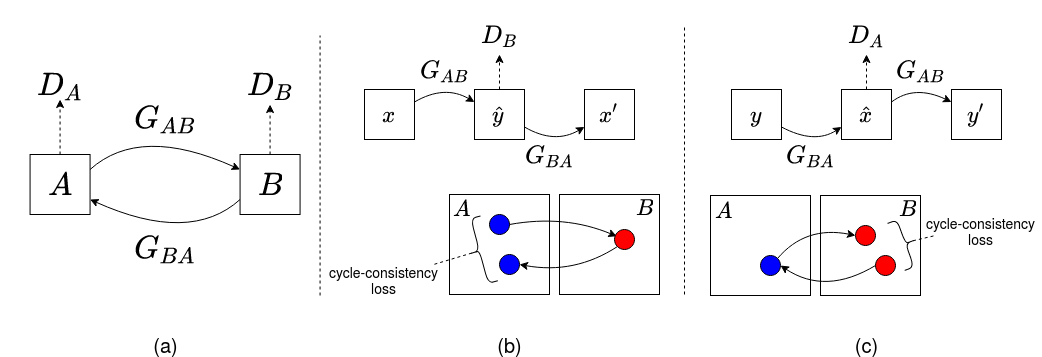
\includegraphics[width=\textwidth]{figures/GANs/cyclegan_concept.png}
    \caption{Simplified representation of CycleGAN training, figure adapted from the original paper \cite{zhu2017unpaired} with notations changed. (a) $G_{AB}$ models \textit{A}$\rightarrow$\textit{B} mapping and $G_{BA}$ its inverse. $D_B$ and $D_A$ are domain \textit{B} and \textit{A} discriminators, respectively. (b) In the \textit{A}$\rightarrow$\textit{B}$\rightarrow$\textit{A} cycle, a domain \textit{A} image $x$ is translated to a representation \textit{$\hat{y} = G_{AB}(x)$} in domain \textit{B}, which is evaluated by $D_B$. It is then used to obtain a reconstruction $x' = G_{BA}(G_{AB}(x))$ of the original image $x$ which is forced by the cycle-consistency to be similar to $x$. (c) The \textit{B}$\rightarrow$\textit{A}$\rightarrow$\textit{B} cycle.}
    \label{fig:cyclegan_concept}
\end{figure}


\subsubsection{CycleGAN-naive: Default CycleGAN applied to HX4-PET synthesis problem}

We investigated unpaired translation of FDG-PET/pCT to HX4-PET using CycleGAN. The term ``unpaired" can be used on two levels here -- on the patient level and on the voxel level. At the patient level, our dataset includes all three image modalities for each patient. The training data for the CycleGAN was patient-level unpaired, meaning the \textit{A}-\textit{B} image correspondence information was not used and both domain \textit{A} and domain \textit{B} samples were independently shuffled. At the voxel level, the registered HX4-PET-reg images provide aligned input-target paired data, whereas the the unregistered images -- HX4-PET-unreg -- are devoid of any artificial deformation related to registration. We, therefore, considered using HX4-PET-unreg images as the set of domain \textit{B} samples which results in CycleGAN training dataset being unpaired at the voxel level as well. The default CycleGAN framework naively applied to our medical image translation problem is henceforth referred to as \textit{CycleGAN-naive}. Figure \ref{fig:cyclegan_naive} shows a schematic of the generator and discriminator training phases of CycleGAN-naive. 

\begin{figure}[h!]
    \centering
    \makebox[\textwidth][c]
    {
        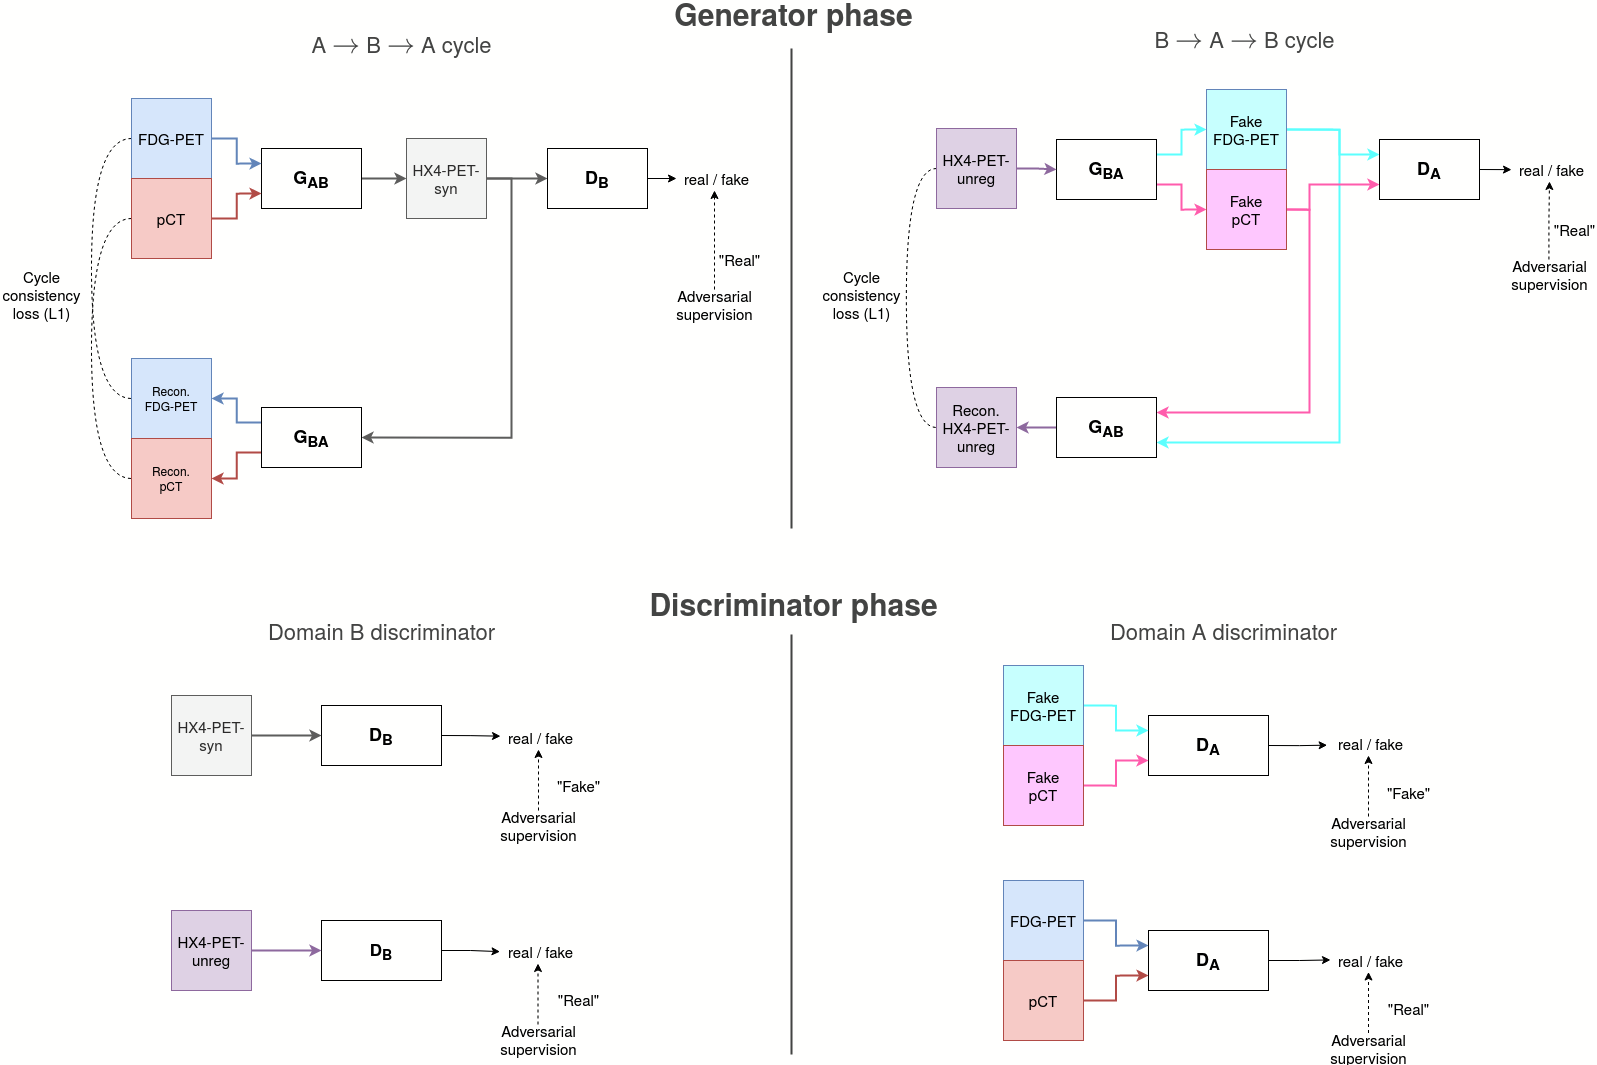
\includegraphics[width=1.5\linewidth]{figures/GANs/CycleGAN-naive.png}
    }
    \caption{CycleGAN-naive training phases. The generators and discriminators are updated in an alternating manner.}
    \label{fig:cyclegan_naive}
\end{figure}{}

We argue that CycleGAN-naive has several drawbacks, and hence, is not an optimal implementation of CycleGAN for our use-case. In the \textit{A}$\rightarrow$\textit{B}$\rightarrow$\textit{A} cycle, $G_{AB}$ takes as input FDG-PET and pCT to output HX4-PET-syn, and $G_{BA}$ uses HX4-PET-syn to reconstruct FDG-PET and pCT. While the task $G_{AB}$ is realistic since hypoxia patterns can be reliably predicted from the inputs and therefore has a physiological basis (see \ref{Related_Work-hypoxia_prediction}), the task $G_{BA}$ is not reasonable. It is not possible to precisely predict a patient's anatomy (CT) as well as their metabolism levels (FDG) from just the hypoxia information, and the CT modality is of more concern here. A CT image contains highly detailed structural information with sharp and fine features, whereas PET images are functional heatmaps having blurred and diffused characteristics. $G_{BA}$ cannot accurately recreate pCT from HX4-PET-syn unless $G_{AB}$ encodes the CT information into the latter in the form of noise. But, then the HX4-PET-syn image would not resemble a clinically acquired HX4-PET scan. Therefore, cycle-consistency constraint conflicts the domain \textit{B} adversarial criterion instead of complementing it. Now looking at the \textit{B}$\rightarrow$\textit{A}$\rightarrow$\textit{B} cycle, the task of $G_{BA}$ is to compute realistic FDG-PET and pCT given only the real HX4-PET-unreg image, which it can perform, especially in pCT, by hallucinating the patient's anatomy. However, in that case, $G_{AB}$ would need to use this fake information to precisely reconstruct the HX4-PET-unreg. Because the task of $G_{AB}$ is to correctly predict hypoxia based on given CT (and FDG-PET) information, it is unreasonable to provide it with fake anatomical information and expect it to predict hypoxia patterns from it that match the real HX4-PET-unreg. Hence, in this cycle as well, cycle-consistency requirement conflicts with adversarial objective. Based on these reasons, we believe that CycleGAN, in its default form, cannot tackle the problem task, and that a more intelligent strategy is required.


\subsubsection{CycleGAN-balanced: An improved design}

We propose a custom design improvement to CycleGAN training to make the system more optimized for our use-case. In PET acquisition, CT scan plays an important role of providing material density information which is used to provide density-correction to the recorded PET intensities. We utilize the fact that an HX4-PET scan is always acquired together with a CT scan which, in our dataset, is a low-dose CT (ldCT). Since the model training is unpaired, the ldCT-unreg images are included in the training data. 

To begin with, we slightly tweak what the domains \textit{A} and \textbf{B} represent here -- let \textit{A} be the domain of FDG-PET images and \textit{B} of HX4-PET images. The CT images -- pCT and ldCT -- are then considered ``supporting" images that provide anatomical context to the generators. Note that pCT has voxel-wise correspondence only with FDG-PET, and ldCT-unreg is aligned only with HX4-PET-unreg. Now, the task of the generators is to take as input a PET image from its source domain and to compute its target domain PET image, while being supplied anatomical context using the available CT image (one that is aligned with the source domain PET). To elaborate on this, let us again consider the two cycles separately: 

\vspace{4mm}
\noindent
\textit{A$\rightarrow$B$\rightarrow$A cycle}: Here, pCT is the available CT image which accompanies the FDG-PET. In \textit{A}$\rightarrow$\textit{B} translation, $G_{AB}$ uses the two images and computes HX4-PET-syn. In \textit{B}$\rightarrow$\textit{A} translation, $G_{BA}$ now \textit{reuses} the pCT as a support image along with the HX4-PET-syn (note that the two are aligned) to reconstruct FDG-PET. The pCT provides the same anatomical context for FDG-PET reconstruction as it did for HX4-PET-syn prediction. The cycle-consistency loss is computed just for the FDG-PET and its reconstructed version. If the HX4-PET-syn represents a plausible hypoxia prediction, then the FDG-PET can be recovered from it up to a great extent since both have an underlying physiological relationship. Therefore, adversarial loss would drive $G_{AB}$ to produce realistic HX4-PET-syn image and the cycle-consistency would encourage this image to be representative of the patient's physiology. 

\vspace{4mm}
\noindent
\textit{B$\rightarrow$A$\rightarrow$B cycle}: In this case, ldCT-unreg is the available CT image that is coupled with the HX4-PET-unreg. In \textit{B}$\rightarrow$\textit{A} translation, $G_{BA}$ uses these two images and computes an equivalent synthetic FDG-PET. In \textit{A}$\rightarrow$\textit{B} translation, $G_{AB}$ reuses the ldCT-unreg and along with the synthetic FDG-PET (note that the ldCT-unreg and the synthetic FDG-PET are aligned), it reconstructs HX4-PET-unreg. Cycle-consistency is applied between the original and reconstructed HX4-PET-unreg. The same ldCT-unreg image provides anatomical context to FDG-PET synthesis and HX4-PET-unreg reconstruction, and if the synthetic FDG-PET represents plausible metabolism patterns, then HX4-PET-unreg can be mostly recovered. In this cycle as well, the adversarial and cycle-consistency objectives would behave in a reinforcing manner.

\vspace{4mm}
The introduction of CT as input to both generators creates a balance between the complexities of the \textit{A}$\rightarrow$\textit{B} and \textit{B}$\rightarrow$\textit{A} mappings since none of them involves predicting fake CT information, all the while still relying on completely unpaired training data. We term this modified design as CycleGAN-balanced. Figure \ref{fig:cyclegan_balanced} shows a schematic of the training phases of its generators and discriminators.

\begin{figure}[h!]
    \centering
    \makebox[\textwidth][c]
    {
        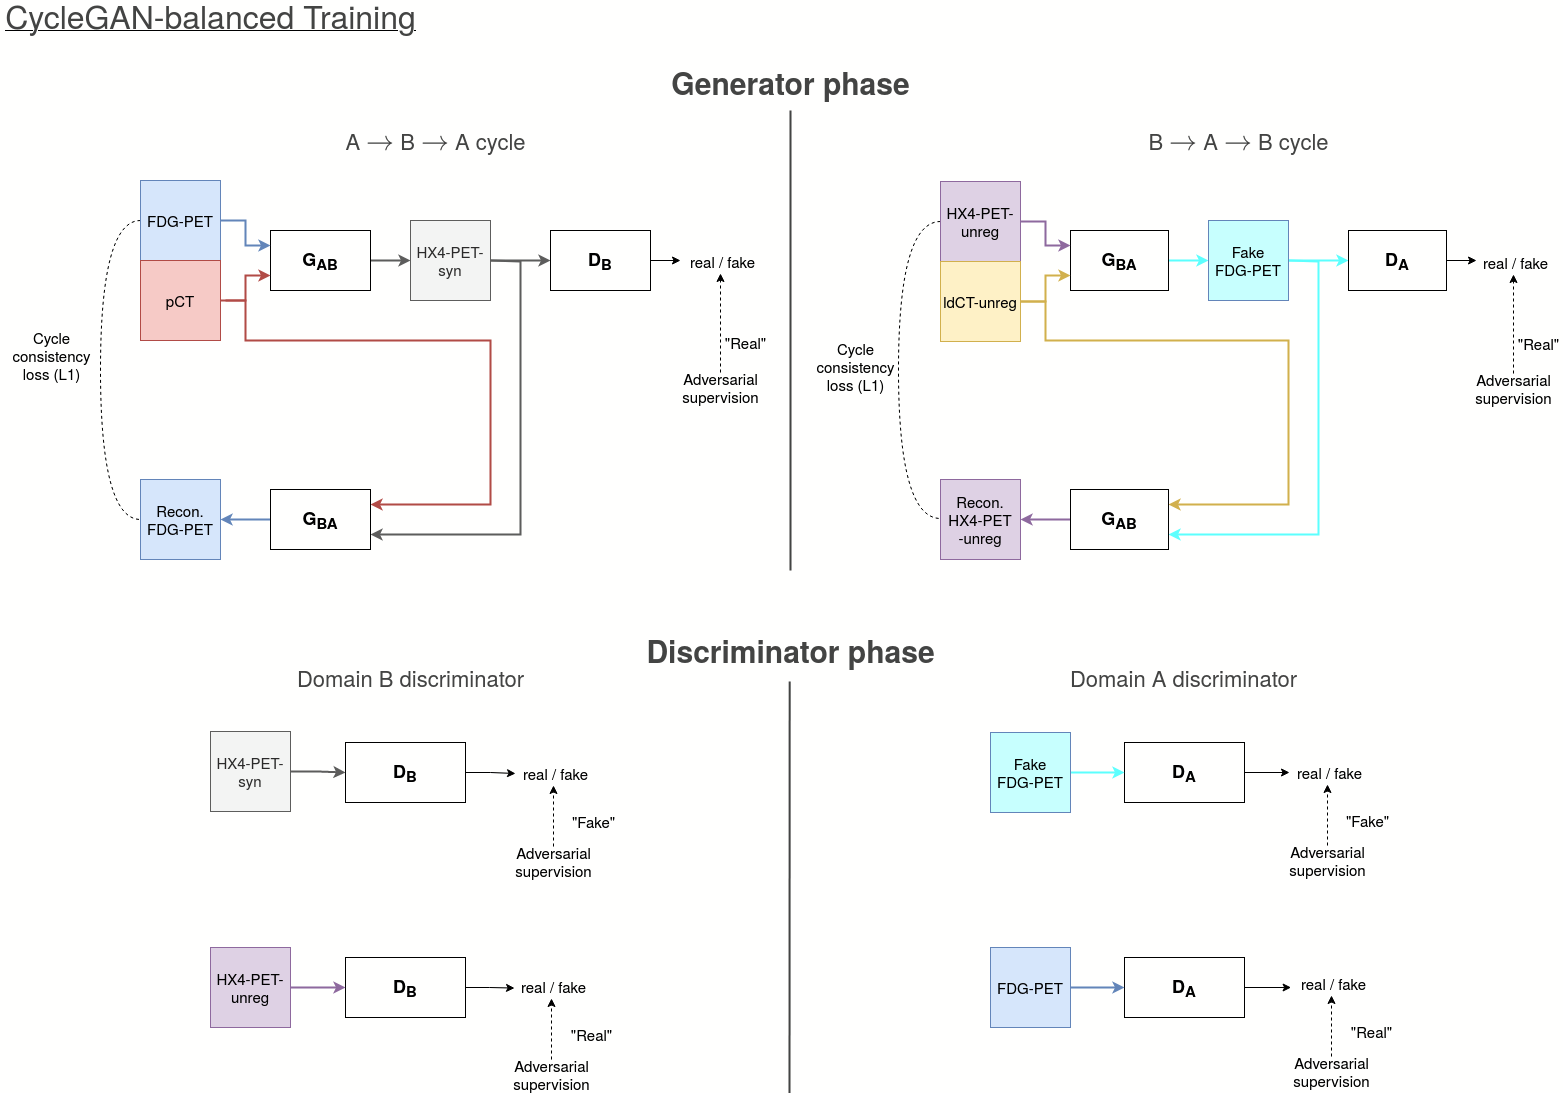
\includegraphics[width=1.5\linewidth]{figures/GANs/CycleGAN-balanced.png}
    }
    \caption{CycleGAN-balanced training phases. \textit{A}$\rightarrow$\textit{B} and \textit{B}$\rightarrow$\textit{A} translation tasks are balanced. In both cases, CT image modality is used only as input to supply anatomical information as a support to the input PET image, and the task of the generator is to predict a single output PET image by combining this information.}
    \label{fig:cyclegan_balanced}
\end{figure}{}


% ---------------------------------------
\subsection{Summary of Data Requirements}
\label{data_requirements}
\todo{Write this}

\begin{figure}[h!]
    \centering
    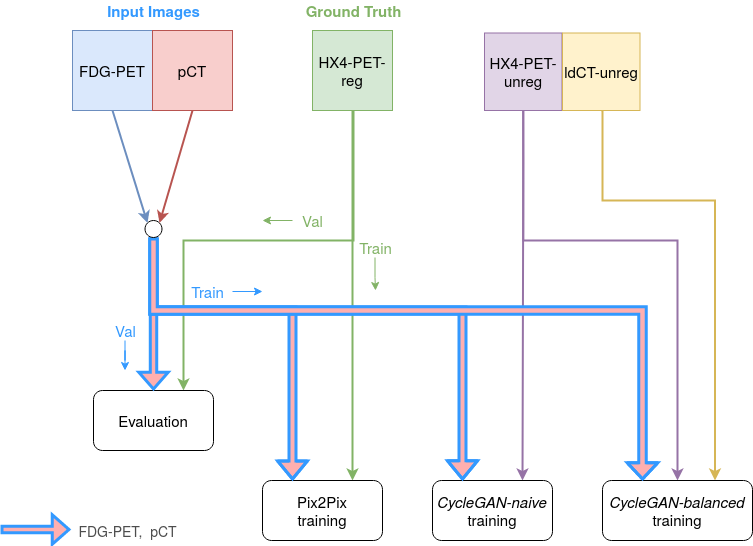
\includegraphics[width=0.95\linewidth]{figures/Data/which_images_where.png}
    \caption{FDG-PET and pCT comprise the model input, which will be supplied to every model during training and validation. HX4-PET-reg is to serve as the ground truth hypoxia map and will be used for validating (and testing) all three models. It will also be used in the supervised training of the Pix2Pix model. The unregistered HX4-PET image will be used in the unpaired training of both the CycleGAN variants. Finally, only \textit{CycleGAN-balanced} will utilize the unregistered ldCT and only during training.}
    \label{fig:which_images_where}
\end{figure}


% -------------------------------
\subsection{Network Architecture}
\label{network_architectures}



%%%%%%%%%%%%%%%%%%%%%%%%%%%%%%%%%%%%%%%%%%%%%%%%%%%%%%%%%%%%%%%%%%%%%%%%%%%%%%%%%%%%%%%%%%%%%%%%%%%%%%%%%%%%%%%%%%%%%%%%%%%%%%%%%%%%%%%%%%%%%%%
\section{Model Training Pipeline}
% HX4-PET SUV normalization with SUVmean_aorta
% Components of the Training Pipeline -- patch based workflow, loss function
% Components of the Validation Pipeline -- patch based workflow, metric computation



%%%%%%%%%%%%%%%%%%%%%%%%%%%%%%%%%%%%%%%%%%%%%%%%%%%%%%%%%%%%%%%%%%%%%%%%%%%%%%%%%%%%%%%%%%%%%%%%%%%%%%%%%%%%%%%%%%%%%%%%%%%%%%%%%%%%%%%%%%%%%%%
\section{Evaluation Methods}



%%%%%%%%%%%%%%%%%%%%%%%%%%%%%%%%%%%%%%%%%%%%%%%%%%%%%%%%%%%%%%%%%%%%%%%%%%%%%%%%%%%%%%%%%%%%%%%%%%%%%%%%%%%%%%%%%%%%%%%%%%%%%%%%%%%%%%%%%%%%%%%
\section{A Simulated Problem: Depth Estimation from Multimodal Input}



